\documentclass[tikz,border=2pt]{standalone}
\usepackage{amsmath,amssymb}
\usetikzlibrary{arrows.meta}
\begin{document}
% AIC and BIC as fit term -2 l-hat plus penalty, n = 100: model A (l-hat = -50, k = 2), model B (l-hat = -48, k = 3).
% AIC: 100 + 4 = 104 vs 96 + 6 = 102 (B smaller); BIC: 100 + 9.21 = 109.21 vs 96 + 13.82 = 109.82 (A smaller).
% Vertical axis starts at 90.
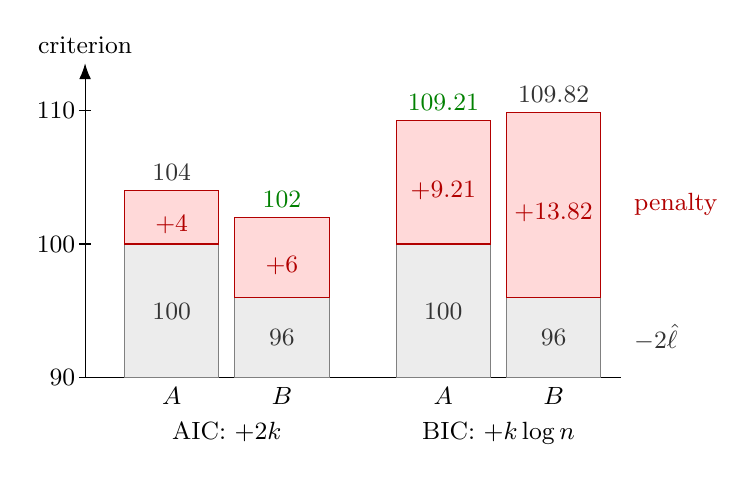
\begin{tikzpicture}[font=\small, >={Latex[length=2mm]}, y=0.17cm]
  \def\bw{1.2}
  % axis (values from 90)
  \draw[->] (-0.5,0) -- (-0.5,23.5) node[above] {criterion};
  \foreach \v in {90,100,110} {
    \draw (-0.58,\v-90) -- (-0.42,\v-90) node[left, xshift=-0.08cm] {$\v$};
  }
  \draw (-0.5,0) -- (6.3,0);
  % bar macro: x, fit, penalty, total label, winner flag
  \newcommand{\critbar}[6]{%
    \fill[gray!15] (#1,0) rectangle (#1+\bw,#2-90);
    \fill[red!15] (#1,#2-90) rectangle (#1+\bw,#2+#3-90);
    \draw[gray] (#1,0) rectangle (#1+\bw,#2-90);
    \draw[red!70!black] (#1,#2-90) rectangle (#1+\bw,#2+#3-90);
    \node[gray!40!black] at (#1+0.5*\bw,0.5*#2-45) {$#2$};
    \node[red!70!black, anchor=base] at (#1+0.5*\bw,#2-90+0.5*#3-1.1) {$#5$};
    \node[#6, anchor=south] at (#1+0.5*\bw,#2+#3-90) {$#4$};
  }
  \critbar{0}{100}{4}{104}{+4}{gray!40!black}
  \critbar{1.4}{96}{6}{102}{+6}{green!50!black}
  \critbar{3.45}{100}{9.21}{109.21}{+9.21}{green!50!black}
  \critbar{4.85}{96}{13.82}{109.82}{+13.82}{gray!40!black}
  % labels under bars
  \foreach \x/\m in {0/A,1.4/B,3.45/A,4.85/B} \node[anchor=north] at (\x+0.5*\bw,0) {$\m$};
  \node[anchor=north] at (1.3,-2.6) {AIC: $+2k$};
  \node[anchor=north] at (4.75,-2.6) {BIC: $+k\log n$};
  % legend-free key
  \node[gray!40!black, anchor=west] at (6.35,3) {$-2\hat\ell$};
  \node[red!70!black, anchor=west] at (6.35,13) {penalty};
\end{tikzpicture}
\end{document}
